\chapter{Математический аппарат квантовой механики}

\begin{sloppypar}
  \section{Состояние и волновая функция. Принцип суперпозиции состояний. Дираковская формулировка квантовой механики. Вектор состояния.}
\end{sloppypar}

В квантовой механике понятие {\em состояния} шире понятия волновой функции, хотя бы потому, что иногда состояния может и не описываться полностью волновой функцией. Например, состояния движущейся частицы описывается ВФ $\Psi(\vr, t)$. Однако, у частицы могут быть и \underline{внутренние степени свободы} (или внутренние динамические переменные). В описании состояния фотона -- элементарной составляющей луча света -- присутствует ещё и поляризация. функция, которая описывает такое состояние не сводится к координатной. Поэтому каждому динамическому состоянию квантовой системы, к том числе не имеющей классических аналогов, будем в дальнейшем сопоставлять некоторый комплексный вектор в абстрактном пространстве. Согласно Дираку (1938~г.), будем обозначать {\em вектор состояния} символом $\ket{\cdots}$. Внутри скобок ставятся буквы или цифры, характеризующие это состояние, например $\ket{\vr}$, $\ket{\vp}$, $\ket{E}$, $\ket{nlm_l}$ и т.д. <<Начинка>> скобок, как правило, состоит из {\em квантовых чисел} (значений динамических переменных, характеризующих состояния системы). В общей квантовой теории эти символы играют ту же роль, что и волновые функции в волновой механике. Более того, теперь в понятие состояния входят не только состояния движения, описываемые переменными пространства, но и они могут зависеть от всех внутренних переменных, не относящихся к движению.

Каким должно быть векторное пространство состояний? Прежде всего оно должно соответствовать основополагающему принципу квантовой механики (или одному из её постулатов) -- {\em принципу суперпозиции состояний}. На языке волновых функций этот принцип можно сформулировать следующим образом.
%
\begin{stmt}[\rom{2} постулат квантовой механики]
Если квантовая система может находиться в состояниях, описываемых волновыми функциями $\Psi_1$ и $\Psi_2$, то она может находиться и в состоянии $\Psi$, описываемом их линейной комбинацией:
$$
\Psi = c_1 \Psi_1 + c_2 \Psi_2, ~~c_1, c_2 \in \mathbb{C}
$$%
%
где $c_1$, $c_2$ -- произвольные (с точностью до условия нормировки) комплексные числа.
\end{stmt}

\begin{figure}[h!]
\centering
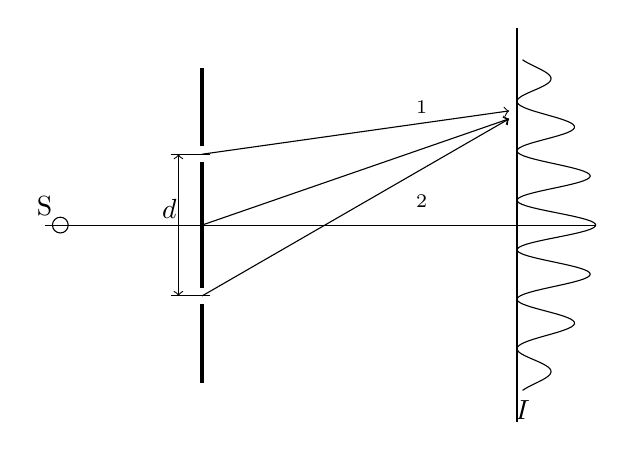
\begin{tikzpicture}[domain=-2:5]
  \draw[-] (-2,0) -- (5,0);
  \draw[very thick] (0, 1) -- (0, 2);
  \draw[very thick] (0, -1) -- (0, -2);
  \draw[very thick] (0, 0.8) -- (0, -0.8);
  \draw[-] (0.1, 0.9) -- (-0.4, 0.9);  
  \draw[-] (0.1, -0.9) -- (-0.4, -0.9);
  \draw[<->] (-0.3, 0.9) -- (-0.3, -0.9);
  \node [left] at (-0.2, 0.2) {$d$};
  \draw [-] (4,2.5) -- (4, -2.5);
  \draw [->] (0, 0.9) -- (3.9, 1.45);
  \node [left] at (3, 1.5) {$\vr_1$};
  \draw [->] (0, -0.9) -- (3.9, 1.35);
  \node [left] at (3, 0.3) {$\vr_2$};
  \draw [->] (0, 0) -- (3.9, 1.35);
  \node [left] at (2.5, 0.6) {$\vr$};
  \draw (-1.8, 0) circle (0.1cm);
  \node[above] at (-2, 0) {S}; 
  \begin{scope}[rotate=-90]
    \draw[domain=-2.1:2.1, samples=200] plot(\x, {cos(0.6*\x r)*cos(5*\x r)^2+4}) node [below] {$I$};
  \end{scope}
\end{tikzpicture}
\caption{К вопросу о суперпозиции состояний.} \label{fig:3_1}
\end{figure}

Этот постулат имеет много наблюдаемых следствий. Одно из них, а именно прохождение электрона через две близко расположенных щели ($\lambdabar_{\text{д.б.}} = \frac{\hbar}{p} \lesssim d$), обсуждается чаще других (см.~\autoref{fig:3_1}). Монохроматический пучок электронов падает на экран слева, проходит сквозь щели в перегородке и затем регистрируется на экране (или фотопластинке) справа. Если поочерёдно закрыть каждую из щелей, то на экране справа мы увидим изображение открытой щели. Но если открыть обе щели одновременно, то вместо изображения двух щелей на фотографии видна система интерференционных полос. Результаты этого опыта можно объяснить, если предположить, что электрон, проходящий через две открытые щели, находится в некотором {\em состоянии суперпозиции}%
%
\begin{equation}
\label{eq:3_1_1}
\Psi(\vr, t) = \brs{\psi_{1}(\vr_1) + \psi_{2}(\vr_2)} e^{-i E t /\hbar}
\end{equation}%
%
Здесь две волны имеют одинаковую частоту $\omega = E/\hbar$, т.к. в противном случае интерференционная картина перестанет быть стационарной. Тогда плотность вероятности нахождения электрона вблизи точки $(\vr, t)$ равна%
%
\begin{equation}
\label{eq:3_1_2}
\begin{gathered}
\abs{\Psi(\vr, t)}^2 = \abs{\psi_1(\vr_1) + \psi_2(\vr_2)}^2
  = \abs{\psi_1}^2 + \abs{\psi_2}^2 + \underbrace{(\psi_1^* \psi_2 + \psi_1 \psi_2^*)}_{2 \Re(\psi_1 \psi_2^*)}= \\
  = \abs{\psi_1}^2 + \abs{\psi_2}^2 + 2\abs{\psi_1}\abs{\psi_2} \cos{(\phi_1 - \phi_2)}
\end{gathered}
\end{equation}%
%
т.е. наблюдается стационарная (не зависящая от времени) интерференционная картина. Последний член в сумме \eqref{eq:3_1_2} представляет интерференцию двух волн вероятности, прошедших в данную точку экрана из разных щелей в перегородке, и зависит от разности фаз волновых функций $\Delta \phi = \phi_1 - \phi_2$. В случае равных по модулю амплитуд вероятности ($\abs{\psi_1} = \abs{\psi_2}$):%
%
\begin{equation}
\label{eq:3_1_3}
\abs{\Psi}^2 = 4 \abs{\psi_1}^2 \cos^2{\frac{\Delta \phi}{2}}
\end{equation}%
%
т.е. интенсивность изображения в разных точках экрана меняется от нуля до $4 \abs{\psi_1}^2$ в зависимости от разности фаз $\Delta \phi$. Например, абсолютный максимум интенсивности расположен на центральной линии при $\Delta \phi = 0$. Может оказаться и так, что при двух открытых щелях на месте изображения одиночной щели мы не обнаружим никакого сигнала, что с корпускулярной точки зрения абсурдно.

% TODO: слишком сумбурный текст
С чем же интерферирует электрон, если вся волновая функция $\Psi$ отнесена к одному электрону? Каждый электрон интерферирует сам с собой, т.к. он вошёл частично в каждую волну и невозможно точно сказать, через какую из щелей он проходит. Если же попытаться установить, через какую фиксированную щель он проходит, поставив дополнительный эксперимент, то интерференционная картина исчезнет. Дело в том, что при этом произойдёт трансформация волновой функции $\psi(\vr_1) \to \psi_1(\vr_1)$, и больше не будет интерференционного состояния.

Таким образом, для сохранения принципа суперпозиции состояний, векторное пространство состояний должно быть линейным, т.е. произвольная линейная композиция двух векторов $\ket{\psi_1}$ и $\ket{\psi_2}$ из этого пространства должна также принадлежать пространству состояний:%
%
\begin{equation}
\label{eq:3_1_4}
\ket{\psi} = c_1\ket{\psi_1} + c_2\ket{\psi_2}, ~~\text{при~} c_1, c_2 \in \mathbb{C}
\end{equation}%
%
% TODO: какой по счёту постулат?
В качестве следствия принципа суперпозиции сделаем следующее замечание%
%
\begin{stmt}[\rom{1} постулат квантовой механики в формализме Дирака]
Квантовое состояние системы полностью определяется вектором состояния $\ket{\psi}$. Векторы $\ket{\psi}$ и $C\ket{\psi} ~(C \neq 0)$ определяют одно и то же состояние.
\end{stmt}%
%
Умножение на число отличное от нуля не меняет состояние, т.е. суперпозиция состояния с самим собой не даёт ничего нового с точки зрения квантовых измерений. В <<начинке>> скобки остаются те же самые квантовые числа -- значения динамических переменных. Это следствие принципа суперпозиции трактуется как первый постулат квантовой механики на основе обобщения экспериментальных фактов. В частности, в опытах по интерференции электронов умножение на константу не меняет распределение волн вероятности, а лишь нормирует интерференционную картинку на общее число частиц в пучке.

Кроме того, векторное пространство состояний обладает обычными свойствами линейного (векторного) пространства:%
%
\begin{enumerate}
\item $\ket{\psi} + \ket{\phi} = \ket{\phi} + \ket{\psi}$ (аксиома коммутативности)
\item $\brs{\ket{\psi} + \ket{\phi}} + \ket{\chi} = \ket{\psi} + \brs{\ket{\phi} + \ket{\chi}}$ (аксиома ассоциативности)
\item $c\brc{\ket{\phi} + \ket{\psi}} = c\ket{\phi} + c\ket{\psi}$ (аксиома дистрибутивности)
\item $(c_1 + c_2)\ket{\psi} = c_1\ket{\psi} + c_2\ket{\psi}$ (аксиома дистрибутивности)
\item $0 \cdot \ket{\psi} \equiv \ket{0} = 0$ (нулевой вектор не описывает никакого состояния квантовой системы. Действительно, если $\ket{\psi} = 0$, то и связанная с этим вектором вероятность найти частицу равна нулю, что означает отсутствие квантового объекта).
\end{enumerate}

Векторное пространство состояний наделено скалярным произведением вектора $\ket{\phi}$ на вектор $\ket{\psi}$, которое в общем случае есть комплексное число $\bk{\phi}{\psi}$. По определению, скалярное произведение выражается через интеграл в конфигурационном пространстве $\vec{q} = (q_1, ..., q_n)$%
%
\begin{equation}
\label{eq:3_1_5}
\bk{\phi}{\psi} = \int \phi^*\underbrace{(q_1, ..., q_n)}_{\vec{q}} \psi\underbrace{(q_1, ..., q_n)}_{\vec{q}} \underbrace{d q_1 ... d q_n}_{d\vec{q}}
\end{equation}%
%
который ещё называется проекцией $\psi$ на $\phi$. Если $\bk{\phi}{\psi} = 0$, то говорят, что функции $\phi$ и $\psi$ ортогональны. Норма $\norm{\psi}$ функции $\psi$ есть скалярное произведение функции на саму себя: $\norm{\psi} = \bk{\psi}{\psi}$.

Основные свойства скалярного произведения:%
%
\begin{enumerate}
  \item Из \eqref{eq:3_1_5}: $\bk{\phi}{\psi} = \bk{\psi}{\phi}^*$, т.е. порядок сомножителей существенен;
%
  \item Если $\ket{\tilde{\phi}} = \lambda_1\ket{\phi}$ и $\ket{\tilde{\psi}} = \lambda_2\ket{\psi}$, то $\bk{\tilde{\phi}}{\tilde{\psi}} = \lambda_1^* \lambda_2 \bk{\phi}{\psi}$, т.е. скалярное произведение линейно по второму и антилинейно по первому сомножителю;
%
  \item норма функции $\psi$ есть неотрицательное вещественное число: $\bk{\psi}{\psi} \geqslant 0$, причём $\bk{\psi}{\psi} = 0$ только если $\ket{\psi} = 0$. Поэтому в математической литературе норма вектора $\ket{\psi}$ определяется как $\norm{\psi} = \sqrt{\bk{\psi}{\psi}}$
\end{enumerate}

Помимо свойства линейности и возможности определения скалярного произведения, пространство состояний обладает ещё и свойством полноты. Это обстоятельность позволяет отождествить его с пространством Гильберта\footnotemark. В нём всегда можно ввести базис как полную ортонормированную систему функций. Следовательно, есть возможность произвольную функцию состояния $\psi(x)$ представить в виде рядов или интегралов, т.е. в виде линейной комбинации базисных функций.
%people
\footnotetext{Давид Гильберт (David Hilbert, 1862-1943)}

Отметим в конечномерной модели аналогию с линейной алгеброй. Пусть вектору состояний $\ket{\psi}$ соответствует двухкомпонентный вектор-столбец $\vec{\psi} = \colvec{2}{\psi_1}{\psi_2}$. Тогда скалярному произведению $\bk{\phi}{\psi}$ можно поставить в соответствие значение%
%
$$
(\phi_1^*, \phi_2^*) \colvec{2}{\psi_1}{\psi_2} = \phi_1^*\psi_1 + \phi_2^* \psi_2
$$%
%
Поэтому наряду с $\psi$ удобно ввести также $\bra{\psi}$ -- аналог комплексно-сопряжённой вектор-строки: $\bra{\psi} \to (\psi_1^*, \psi_2^*)$. Данный объект есть элемент дуального (или сопряженного) векторного пространства, хорошо известного в линейной алгебре. Операцию перехода к элементам дуального векторного пространства обозначим символом $^\dag$, так что%
%
$$
\bra{\psi} = \ket{\psi}^\dag
$$%
%
В терминах матриц это означает эрмитово\footnotemark сопряжение, т.е. операцию транспонирования и комплексного сопряжения. Таким образом, для любого вектора состояний $\ket{\psi}$, принадлежащего гильбертову пространству ($\ket{\psi} \in \mathbb{H}$), вектор дуального пространства $\bra{\phi} \in \mathbb{H}^*$ задаёт линейный функционал, аргумент которого сам вектор $\ket{\psi}$, а его значение $\bk{\phi}{\psi} \in \mathbb{C}$.
%people
\footnotetext{Шарль Эрмит (Charles Hermite, 1822-1901)}
%
Вектор $\ket{\psi}$ называют {\em кет-вектором}, а вектор $\bra{\psi}$ дуального пространства -- {\em бра-вектором}. Дело в том, что эти обозначения, введённые Дираком, соответствуют английскому слову <<bracket>> -- скобка. <<Скобка>> (скалярное произведение) $\bk{\phi}{\psi}$ состоит из двух векторов: <<бра>> и <<кет>>.

В заключение этого параграфа ещё раз обратимся к принципу суперпозиции состояний, записанному в векторных обозначениях в виде \eqref{eq:3_1_4}:%
%
$$
\ket{\psi} = c_1 \ket{\psi_1} + c_2 \ket{\psi_2}
$$%
%
тогда:%
%
$$
\bra{\psi} = c_1^* \bra{\psi_1} + c_2^* \bra{\psi_2}
$$%
%
Поскольку ранее мы договорились описывать состояния функциями нормированными на единицу, то для всех векторов состояний принимаем норму%
%
$$
\bk{\psi}{\psi} = \bk{\psi_1}{\psi_1} = \bk{\psi_2}{\psi_2} = 1
$$%
%
отсюда:%
%
$$
\bk{\psi}{\psi} = \abs{c_1}^2 + \abs{c_2}^2 + 2 \Re{c_1^* c_2 \bk{\psi_1}{\psi_2}} = 1
$$%
%
Выбирая состояния $\ket{\psi_1}$ и $\ket{\psi_2}$ взаимно ортогональными, т.е. $\bk{\psi_1}{\psi_2} = 0$, получим $\abs{c_1}^2 + \abs{c_2}^2 = 1$. В таком случае коэффициенты линейной комбинации \eqref{eq:3_1_4} имеют вполне определённый физический смысл: $\abs{c_1}^2$ ($\abs{c_2}^2$) -- вероятность обнаружить систему в состоянии $\ket{\psi_1}$ ($\ket{\psi_2}$). Мы получили важное дополнение к принципу суперпозиции состояний

\begin{stmt}
Если измерение в состоянии \circled{1} даёт результат \circled{1}, а измерение в состоянии \circled{2} даёт результат \circled{2}, то измерение в суперпозиции этих состояний даёт либо результат \circled{1}, либо результат \circled{2}.
\end{stmt}

Термин <<квантовая суперпозиция>> означает, что при измерении нельзя получить <<что-то третье>>, а лишь только <<первое>> или <<второе>> с той или иной вероятностью. В этом заключена ещё одна сторона статистической интерпретации волновой функции в квантовой механике.

\section{Наблюдаемые и операторы физических величин. Линейные и эрмитовы операторы}

В квантовой механике каждой физической величине $F$ (или {\em наблюдаемой} $F$, по терминологии Дирака), ставится в соответствие линейный оператор $\op{F}$, действующий в пространстве векторов состояний $\ket{\psi}$, описывающих состояния физической системы. Линейный оператор $\op{F}$ задаёт в гильбертовом пространстве $\mathbb{H}$ некоторое линейное отображение некоторого множества $D_{\op{F}}$ (области определения $\op{F}$) в множество значений $R_{\op{F}}$:

$$
\ket{\phi} = \op{F} \ket{\psi} \in R_{\op{F}}, ~~\text{где}~~ \ket{\psi} \in D_{\op{F}}
$$

\begin{defn}
Оператор $\op{F}$ называется \underline{линейным}, если для него выполняется:
\begin{equation}
  \label{eq:3_2_1}
	\op{F}(c_1 \ket{\psi_1} + c_2 \ket{\psi_2}) = c_1 \op{F}\ket{\psi_1} + c_2 \op{F}\ket{\psi_2}
\end{equation}%
где $\ket{\psi_1}, \ket{\psi_2} \in D_{\op{F}}$, а $c_1, c_2 \in \mathbb{C}$.
\end{defn}

В линейности оператора $\op{F}$ физической величины $F$ находит отражение принцип суперпозиции состояний, т.к. он с самого начала заложен в квантовую теорию. По своему определению это оператор, который переводит линейную комбинацию (суперпозицию) одних векторов состояний в линейную комбинацию других векторов состояний:%
%
$$
c_1 \ket{\psi_1} + c_2\ket{\psi_2} \xrightarrow{~~\op{F}~~} c_1 \ket{\phi_1} + c_2 \ket{\phi_2}
$$%
%
Таким образом, применение линейных операторов не нарушает принципа суперпозиции состояний.

Линейные операторы образуют алгебру, т.е. множество, для которых справедливы следующие свойства:

%--
% Начинаются свойства
%--

\begin{enumerate}
%
  \item\label{prop:op:1} Умножение на комплексное число:
  $$
  (c\op{F}) \ket{\psi} \equiv 
    \underbrace{\left. c (\op{F} \ket{\psi}) \right|_{\text{\eqref{eq:3_2_1}}} =
    \op{F} (c \ket{\psi})}_{\text{свойство однородности $\op{F}$}}
  $$

  \item Коммутативность операции сложения:
  $$
  \begin{gathered}
  (\op{F} + \op{G})\ket{\psi} \equiv
    \underbrace{
      \op{F}\ket{\psi} + \op{G}\ket{\psi}  = \op{G}\ket{\psi} + \op{F}\ket{\psi}
    }_{\text{из аксиомы коммутативности}}
    = (\op{G} + \op{F})\ket{\psi}\\ 
    \Rightarrow~~ \op{F} + \op{G} = \op{G} + \op{F}
  \end{gathered}
  $$

  \item Произведение операторов:
  $$
  \op{P} = \op{F}\op{G} ~~\Rightarrow~~ \op{P}\ket{\psi} = \op{F}(\op{G}\ket{\psi})
  $$
  В общем случае операция произведения некоммутативна: $\op{F}\op{G}\ket{\psi} \neq \op{G}\op{F}\ket{\psi}$
%
\end{enumerate}

%--
% Вводим дополнительное определение
%--

\begin{defn}
Разность $\op{F}\op{G} - \op{G}\op{F}$ называется \underline{коммутатором} операторов $\op{F}$ и $\op{G}$ и обозначается квадратными скобками:%
%
\begin{equation}
\label{eq:3_2_2}
\brs{\op{F}, \op{G}} \equiv \op{F}\op{G} - \op{G}\op{F}
\end{equation}%
%
Говорят, что операторы \underline{коммутируют}, если $\brs{\op{F}, \op{G}} = 0$.
\end{defn}%
%
\noindent
Из свойства~\ref{prop:op:1} следует, что любой оператор коммутирует с константой: $[\op{F}, C] = 0$.

%--
% Продолжаем список
%--

\begin{enumerate}
%
  \setcounter{enumi}{3}
  %
  \item Пусть $\ket{\phi} = \op{F}\ket{\psi}$. Если имеется взаимно однозначное соответствие между векторами $\ket{\psi}$ и $\ket{\phi}$, то оно определяет два линейных оператора $\op{F}$ и $\op{G}$:
  $$
  \ket{\phi} = \op{F}\ket{\psi} ~~~~~ \ket{\psi} = \op{G}\ket{\phi}
  $$
  При этом операторы $\op{F}$ и $\op{G}$ по определению обратны друг к другу, т.е. удовлетворяют операторным уравнениям%
  %
  \begin{equation}
  \label{eq:3_2_3}
  \op{F}\op{G} = \op{G}\op{F} = 1
  \end{equation}%
%
\end{enumerate}

\noindent
% TODO: дать конкретную ссылку на главу
Эти два определение обратных операторов эквивалентны. Оператор, обратный данному, существует не всегда\footnote{Это прояснится в дальнейшем при рассмотрении матричного представления операторов: обратную имеет только невырожденная матрица, т.е. с отличным от неля определителем}. Когда он существует, его обозначают символом $\op{F}^{-1}$, и альтернативным определению \eqref{eq:3_2_3} будет

\begin{equation}
\label{eq:3_2_3_add}
\op{F}\op{F}^{-1} = \op{F}^{-1}\op{F} = 1
\tag{\ref{eq:3_2_3}$'$}
\end{equation}%
%
Если операторы $\op{F}$ и $\op{G}$ имеют обратные, тогда существует и обратный оператор из произведения: 

\begin{equation}
\label{eq:3_2_4}
(\op{F}\op{G})^{-1} = \op{G}^{-1} \op{F}^{-1}
\end{equation}%
%
Отметим перестановку сомножителей в правой части \eqref{eq:3_2_4}.

\begin{excr}
Доказать \eqref{eq:3_2_4}, используя \eqref{eq:3_2_3_add}.
\end{excr}

Рассмотрим наряду с оператором  $\op{F}$, действующем в пространстве состояний $\mathbb{H}$, оператор $\op{F}^\dag$, действующий в сопряжённом пространстве $\mathbb{H}^*$. Пусть $\ket{\chi} = \op{F}\ket{\psi}$, тогда по определению вектор в $\mathbb{H}^*$ получается эрмитовым сопряжением:
$$
\ket{\chi}^\dag = \left. (\op{F}\ket{\psi})^\dag \right|_{(\op{A}\op{B})^\dag = \op{B}^\dag \op{A}^\dag} = \bra{\psi} \op{F}^\dag
$$

\begin{equation}
\label{eq:3_2_5}
\boxed{
	\bra{\chi} = \bra{\psi} \op{F}^\dag
}
\end{equation}

% TODO: мутные выкладки, разобраться
Оператор $\op{F}^\dag$ эрмитово сопряжён по отношению к оператору $\op{F}$ и действует <<справа налево>>. В результате действия $\op{F}^\dag$ на бра-вектор $\bra{\psi}$ получается бра-вектор $\bra{\chi}$. К ному можно справа <<приставить>> некоторый вектор $\ket{\phi} \in \mathbb{H}$. А это значит, формально можно считать, что оператор $\op{F}^\dag$ действует не только <<налево>>, но и <<направо>>, т.е. на $\ket{\phi}$. Тогда, получим%
%
$$
\bfk{\psi}{\op{F}^\dag}{\phi} = \bk{\chi}{\phi} = \bk{\phi}{\chi}^*
$$%
%
Следовательно, из \eqref{eq:3_2_5}:%
%
\begin{equation}
\label{eq:3_2_6}
\boxed{
  \bfk{\psi}{\op{F}^\dag}{\phi} = \bfk{\phi}{\op{F}}{\psi}^*
}
\end{equation}

\begin{defn}
Эрмитово сопряжённым к $\op{F}$ называется оператор $\op{F}^\dag$, удовлетворяющий \eqref{eq:3_2_6}.
\end{defn}

Для эрмитово сопряжённых операторов легко убедиться в справедливости соотношений:
$$
\begin{gathered}
(c\op{F})^\dag = c^* \op{F}^\dag \\
(\op{F}^\dag)^\dag = \op{F} \\
(\op{F} + \op{G})^\dag = \op{F}^\dag + \op{G}^\dag \\
(\op{F}\op{G})^\dag = \op{G}^\dag \op{F}^\dag
\end{gathered}
$$

\begin{excr}
Доказать приведённые выше свойства.
\end{excr}

\begin{defn}
Если $\op{F}^\dag = \op{F}$ или
\begin{equation}
\label{eq:3_2_7}
\forall \ket{\psi},\ket{\phi} \in D_{\op{F}} ~~\to~~
	\bfk{\psi}{\op{F}}{\phi} = \bfk{\phi}{\op{F}}{\psi}^*
\end{equation}
то оператор $\op{F}$ называется \underline{эрмитовым} или сопряжённым самому себе (\underline{самосопряжённым}).
\end{defn}

В литературе иногда используется другое эквивалентное определение эрмитово сопряжённого оператора. Пусть $\ket{\psi}$ и $\ket{\phi}$ -- два произвольных вектора состояний, $\op{F}\ket{\psi} \equiv \ket{\op{F}\psi}$. Тогда оператор $\op{F}^\dag$ называется эрмитово сопряжённым по отношению к оператору $\op{F}$, если оба оператора имеют одну и ту же область определения и выполняется равенство
\begin{equation}
\label{eq:3_2_6_add}
\boxed{
	\bk{\phi}{\op{F}\psi} = \bk{\op{F}^\dag\phi}{\psi}
} = \bk{\psi}{\op{F}^\dag \phi}^*
\tag{\ref{eq:3_2_6}$'$}
\end{equation}
или
\begin{equation}
\label{eq:3_2_6_add_x2}
\boxed{
	\bk{\psi}{\op{F}^\dag \phi} = \bk{\op{F} \psi}{\phi}
}
\tag{\ref{eq:3_2_6}$''$}
\end{equation}
что эквивалентно:
$$
\int \psi^*(\vec{q}) \op{F}^\dag \phi(\vec{q})\diff\vec{q}
  = \int \brc{\op{F} \psi(\vec{q})}^* \phi(\vec{q})\diff\vec{q}
$$

\begin{defn}
$\op{F}$ называется \underline{эрмитовым} (самосопряжённым), если $\op{F}^\dag = \op{F}$, т.е.:
\begin{equation}
\label{eq:3_2_7_add}
\forall \ket{\psi}, \ket{\phi} \in D_{\op{F}}  ~\to~ \boxed{ \bk{\psi}{\op{F} \phi} = \bk{\op{F}\psi}{\phi} }
\tag{\ref{eq:3_2_7}$'$}
\end{equation}
или
$$
\int \psi^*(\vec{q}) \op{F} \phi(\vec{q})\diff\vec{q}
  = \int \brc{\op{F} \psi(\vec{q})}^* \phi(\vec{q})\diff\vec{q}
$$
\end{defn}

Здесь область определения $D_{\op{F}}$ включает все векторы состояний $\ket{\psi}$ и $\ket{\phi}$, для которых
\begin{enumerate}
\item $\norm{\psi} < \infty$, $\norm{\phi} < \infty$
\item $\norm{\op{F} \psi} < \infty$, $\norm{\op{F} \phi} < \infty$
\end{enumerate}


\begin{defn}
Выражение:
$$
\bk{\phi}{\op{F}\psi} \equiv
  \bfk{\phi}{\op{F}}{\psi} =
  \int \phi^*(\vec{q})\op{F}\psi(\vec{q})\diff\vec{q}
$$
называется \underline{матричным элементом} оператора $\op{F}$ на функциях $\phi$ и $\psi$, или матричным элементом $\op{F}$ <<в обкладках>> векторов $\bra{\phi}$ и $\ket{\psi}$.

Величина $\bk{\psi}{\op{F}\psi} \equiv \bfk{\psi}{\op{F}}{\psi}$ называется \underline{диагональным матричным элементом}.
\end{defn}

Из \eqref{eq:2_2_1} оператора $\op{F}$ физической величины следует, что наблюдаемое значение $\avg{F}$ физической величины $F$ (её среднее или ожидаемое значение) совпадает с диагональным матричным элементом
\begin{equation}
\label{eq:3_2_8}
\boxed {
	\avg{F} = \bk{\psi}{\op{F}\psi} = \bfk{\psi}{\op{F}}{\psi}
}
\end{equation}%
%
В квантовой механике средние значения физических величин в любом состоянии представляют собой измеряемые, а следовательно, действительные числа: $\avg{F} = \avg{F}^*$, или, в соответствии с \eqref{eq:3_2_8}:
\begin{equation}
\label{eq:3_2_9}
\bfk{\psi}{\op{F}}{\psi}
  = \left .\bfk{\psi}{\op{F}}{\psi}^* \right|_{\text{\eqref{eq:3_2_6}, \eqref{eq:3_2_7}}}
  = \bfk{\psi}{\op{F}^\dag}{\psi}
\end{equation}%
%
или $\op{F}^\dag = \op{F}$. То есть физическим (наблюдаемым) величинам соответствуют \underline{эрмитовы операторы}.

Таким образом, в квантовой механике каждой физический величине $F$ сопоставляется линейный и эрмитов оператор $\op{F}$, выбираемый так, чтобы среднее из многих измерений этой величины $\avg{F}$ в состоянии, описываемом функцией $\Psi(\vr, t)$, было равно
$$
\avg{F} = \bfk{\Psi}{\op{F}}{\Psi}
$$
Здесь функция $\Psi(\vr, t)$ является вектором пространства Гильберта и удовлетворяет условию нормировки $\bk{\Psi}{\Psi} = 1$.

Об измеряемой величине $F$, помимо её среднего значения $\avg{F}$, судят ещё по её среднему квадратичному отклонению от $\avg{F}$ (дисперсии)

\begin{equation}
\label{eq:3_2_10}
\avg{(\Delta F)^2} \equiv \avg{(F - \avg{F})^2}
\end{equation}%
%
Пользуясь общим определением \eqref{eq:2_2_1} среднего значения, получим

\begin{equation}
\label{eq:3_2_11}
\avg{(\Delta F)^2} = \bfk{\psi}{(\op{F} - \avg{F})^2}{\psi}
\end{equation}%
%
Т.к. оператор $\op{F}$ -- эрмитов, а $\avg{F}$ -- действительное число, то оператор $\op{F} - \avg{F}$ -- также эрмитов, поэтому

\begin{equation}
\label{eq:3_2_12}
\begin{gathered}
\left. \avg{(\Delta F)^2} \right|_{\text{\eqref{eq:3_2_7_add}}} =
  \bk{(\op{F} - \avg{F})\psi}{(\op{F} - \avg{F})\psi} = \\ =
  \int \abs{\brc{\op{F} - \avg{F}}\psi}^2\diff\vec{q} \geqslant 0
\end{gathered}
\end{equation}

Следовательно, чтобы величина $F$ не имела разброса в состоянии $\ket{\psi}$, т.е. чтобы $\avg{(\Delta F)^2} = 0$, необходимо выполнение условия

\begin{equation}
\label{eq:3_2_13}
\op{F}\ket{\psi} = \avg{F}\ket{\psi}
\end{equation}

Таким образом, условие $\avg{(\Delta F)^2} = 0$ выполняется, если состояние $\ket{\psi}$ является собственным для оператора $\op{F}$ (см.~\sref{3}{2}). При $\avg{F} = f$ этому условию удовлетворяют собственные вектора оператора $\op{F}$, для которых вместо \eqref{eq:2_3_2} можно записать

\begin{equation}
\label{eq:3_2_14}
\op{F}\ket{\psi_{f}} = f \ket{\psi_{f}}
\end{equation}%
%
где $f$ -- собственные значения оператора $\op{F}$.

Поэтому далее будем считать, что никаких значений величины $F$ нельзя наблюдать на опыте, кроме тех, которые являются собственными значениями оператора $\op{F}$. Иными словами, в квантовой механике постулируется:
\begin{stmt}[\rom{3} постулат квантовой механики]
Физическая величина $F$ в любом квантовом состоянии может принимать только те значения, которые принадлежат спектру её оператора $\op{F}$.
\end{stmt}

Наблюдаемые на опыте величины вещественны, значит, должны быть вещественными собственные значения $f$ оператора $\op{F}$ в \eqref{eq:3_2_14}. Докажем теорему

\begin{thm}
Если оператор $\op{F}$ эрмитов, то он имеет вещественные собственные значения.
\end{thm}
%
\begin{proof}
Применим к левой части \eqref{eq:3_2_14} условие эрмитовости \eqref{eq:3_2_7} оператора $\op{F}$:

$$
\left. \bfk{\psi_f}{\op{F}}{\psi_f}^* \right|_{\text{\eqref{eq:3_2_7}}} =
  \bfk{\psi_f}{\op{F}}{\psi_f}
$$%
%
Отсюда:

$$
f^*\bk{\psi_f}{\psi_f}^* = f^* \bk{\psi_f}{\psi_f} = f\bk{\psi_f}{\psi_f}
$$
Или $\boxed{f^* = f}$, что и требовалось доказать.
\end{proof}

Этим полностью разъясняется роль эрмитовых операторов для квантовой механики: эрмитовы операторы изображают вещественные (наблюдаемые) величины. Поэтому в современной англоязычной литературе часто эрмитовы операторы называют наблюдаемыми (\textit{observables}).

\section{Условие ортогональности и полноты для собственных функций операторов физических величин}

Уравнение \eqref{eq:2_3_3} на собственные значения $\op{F}$ для дискретного спектра в терминах собственных векторов принимает вид

\begin{equation}
\label{eq:3_3_1}
\op{F}\ket{\psi_n} = f_n \ket{\psi_n} ~~\text{или}~~ \op{F}\ket{n} = f_n\ket{n}
\end{equation}
где $\psi_n \equiv \ket{n}$, $n = 0, 1, 2, ...$

Может оказаться так, что каждому собственном значению (СЗ) $f_n$ отвечает один собственный вектор. В таком случае говорят о невырожденном (или простом) спектре оператора $\op{F}$. Может быть и так, что $f_n$ соответствует несколько собственных векторов, например
$$
f_n \to \brcr{\ket{\psi_n^{(1)}}, \ket{\psi_n^{(2)}}, ..., \ket{\psi_n^{(g)}} }
$$%
%
Такое собственное значение называется вырожденным и говорят о вырожденном спектре оператора $\op{F}$. 

\begin{defn}
Максимальное количество линейно-независимых собственных векторов (собственных функций), отвечающих данному собственному значению, называется \underline{кратностью вырождения} этого собственного значения.
\end{defn}

\begin{stmt}
Собственные функции (собственные векторы) эрмитова оператора, отвечающие различным собственным значениям, взаимно ортогональны.
\end{stmt}
%
\begin{proof}

Рассмотрим случай, когда вырождение отсутствует. Имеем:

\begin{equation}
  \label{eq:3_3_2}
	\op{F}\ket{\psi_n} = f_n \ket{\psi_n},~~~
  \op{F}\ket{\psi_m} = f_m \ket{\psi_m},~~~
  f_n \neq f_m
\end{equation}

Умножим первое уравнение из \eqref{eq:3_3_2} скалярно на $\bra{\psi_m}$, второе уравнение -- на $\bra{\psi_n}$, и вычтем из первого уравнения комплексно сопряжённое второе:
$$
\left.
  \bfk{\psi_m}{\op{F}}{\psi_n} - \bfk{\psi_n}{\op{F}}{\psi_m}^\dag
      \right|_{\text{\eqref{eq:3_2_7}}} = 0 =
  f_n \bk{\psi_m}{\psi_n} - \underbrace{f_m^*}_{= f_m} \bk{\psi_n}{\psi_m}^*
$$%
%
Из вещественности собственных значений $\op{F}$ получаем

\begin{equation}
\label{eq:3_3_3}
(f_n - f_m) \bk{\psi_m}{\psi_n} = 0
\end{equation}%
%
Т.к. по условию $f_m \neq f_n$, то $\boxed{\bk{\psi_m}{\psi_n} = 0}$, что и требовалось доказать.
\end{proof}

Т.к. функции дискретного спектра мы может нормировать к единице

\begin{equation}
\label{eq:3_3_4}
\bk{\psi_n}{\psi_n} = 1
\end{equation}%
%
это равенство можно объединить с равенством \eqref{eq:3_3_3}:

\begin{equation}
\label{eq:3_3_5}
\boxed{
	\bk{\psi_m}{\psi_n} = \bk{m}{n} = \delta_{mn}
}
\end{equation}%
%
В дальнейшем мы будем считать, что собственные векторы линейного эрмитовa оператора образуют ортонормированную системы векторов.

Собственные векторы $\brcr{\ket{\psi_n^{(i)}}} ~~ i = \overline{1,g}$, соответствующие вырожденному СЗ $f_n$, вообще говоря, не являются взаимно ортогональным (см., например, \eqref{eq:3_3_3} при $f_n = f_m$). Любая линейная комбинация этих векторов

\begin{equation}
\label{eq:3_3_6}
\ket{\psi_n^s} = \sum_{i=1}^{g} c_i^{(s)} \ket{\psi_n^{(i)}}
\end{equation}%
%
также будет собственным вектором оператора $\op{F}$ с тем же СЗ $f_n$. Из линейной алгебры известно, что линейные комбинации \eqref{eq:3_3_6} можно выбрать так, чтобы все векторы нового набора $\brcr{\ket{\psi_n^{(s)}}}, s = \overline{1,g}$ составляли ортонормированную систему (например, с помощью процедуры ортогонализации по Шмидту). Таким образом, даже в случае вырожденного спектра эрмитова оператора $\op{F}$ все его собственные векторы можно считать ортонормированными.

В математике доказывается, что системы всех ортонормированных собственных векторов линейного эрмитова оператора с дискретным спектром является полным набором в гильбертовом пространстве состояний, а значит, ортонормированным базисом этого пространства.

Следовательно, $\forall \ket{\psi} \in \mathbb{H}$ мы может разложить его по системе собственных векторов оператора $\op{F}$:

\begin{equation}
\label{eq:3_3_7}
\ket{\psi} = \sum_n c_n \ket{\psi_n}
\end{equation}%
%
где%
%
$$
\bk{\psi_m}{\psi} =
  \sum_n c_n \underbrace{
    \bk{\psi_m}{\psi_n}
  }_{
    \mathclap{=\delta{mn}~(\text{из \eqref{eq:3_3_5}})}
  } = \sum_n c_n \delta_{mn} = c_m
$$%
%
т.е. $\boxed{c_n = \bk{\psi_n}{\psi}}$ -- коэффициенты $c_n$ разложения \eqref{eq:3_3_7} есть проекции вектора $\ket{\psi}$ на соответствующие собственные вектора оператора $\op{F}$.

С помощью $\ket{\psi}$ прямого пространства и $\bra{\phi}$ сопряжённого было определено число -- скалярное произведение этих векторов $\bk{\phi}{\psi}$. Однако, скалярное произведение -- не единственный способ перемножения векторов бра и кет. Можно составить произведение

\begin{equation}
\label{eq:3_3_8}
\op{P}_{\psi} = \proj{\psi}{\phi}
\end{equation}%
%
которое обладает свойствами оператора. Действительно, оператор ставит в соответствие произвольному вектору $\ket{\chi}$ некоторый другой вектор по определённому правилу:

\begin{equation}
\label{eq:3_3_9}
\op{P}_\psi \ket{\chi} = \ket{\psi} \underbrace{\bk{\phi}{\chi}}_{= c} = c \ket{\psi}
\end{equation}%
%
Как видим, конструкция \eqref{eq:3_3_8} обладает свойствами оператора проектирования: при действии на произвольный вектор $\ket{\chi}$ она переводит его в вектор $\ket{\psi}$ с числовым множителем $c$, или проектирует произвольное состояние $\ket{\chi}$ на $\ket{\psi}$ с весовым множителем $c$.

Теперь вернёмся к разложению \eqref{eq:3_3_7} и подставим в него явный вид коэффициентов $c_n$:

\begin{equation}
\label{eq:3_3_10}
\ket{\psi} = \sum_n \ket{\psi_n} \bk{\psi_n}{\psi} =
  \brc{\sum_n \proj{\psi_n}{\psi_n}} \ket{\psi}
\end{equation}%
%
Отсюда видно, что выражение в скобках должно быть единичным оператором

\begin{equation}
\label{eq:3_3_11}
\boxed {
	\sum_n \proj{\psi_n}{\psi_n} = \mathds{1}
}
\end{equation}

Полученное соотношение \eqref{eq:3_3_11} называется условием полноты системы собственных векторов оператора $\op{F}$. (Иногда левую часть равенства \eqref{eq:3_3_11} называют операторным разложением единицы по отношению к собственным векторам оператора $\op{F}$.) Объясним смысл термина <<условие полноты>>. Возьмём одно слагаемое из суммы $\proj{\psi_n}{\psi_n}$ и подействуем этим оператором на вектор $\ket{\psi}$, получим

\begin{equation}
\label{eq:3_3_12}
\ket{\psi_n} \underbrace{\bk{\psi_n}{\psi}}_{ = c_n} \equiv
  \op{P}_n \ket{\psi} = c_n \ket{\psi_n}
\end{equation}%
%
где, как и ранее, $c_n = \proj{\psi_n}{\psi_n}$. Таким образом, $\op{P}_n$ -- это проектор (оператор проектирования) произвольного вектора состояния $\ket{\psi}$ на одномерное подпространство, натянутое на орт $\ket{\psi_n}$. В силу полноты системы собственных векторов $\brcr{\ket{\psi_n}}$ сумма подобных проекторов должна представлять собой проектор на всё гильбертово пространство $\mathbb{H}$, т.е., очевидно, единичный оператор.

Сформулируем основные свойства проекторов

\begin{enumerate}
\item оператор $\op{P}_n$ -- эрмитов;
\item $\op{P}_n^2 = \op{P}_n$; ~~\footnotemark
\item собственные значения $\op{P}_n$: $\lambda = \brcr{0, 1}$
\end{enumerate}

\begin{excr}
Доказать вышеперечисленные свойства.
\end{excr}

\footnotetext{
  Сколь физична вырожденная матрица? Иными словами, имеет ли физический смысл оператор, не имеющий обратного?

  У проектора $\op{P}_n$ нет обратного оператора. Действительно, если бы он был, то из
  $$
  \op{P}_n^2 = \op{P}_n  ~~\to~~
    \op{P}_n \underbrace{\op{P}_n \op{P}^{-1}_n}_{\mathds{1}} = 
      \underbrace{\op{P}_n \op{P}^{-1}_n}_{\mathds{1}}
  $$%
  %
  или $\op{P}_n = \mathds{1}$, что в общем случае противоречит определению оператора $\op{P}_n$.

  Однако оператор $\op{P}_n$ -- эрмитов, а значит физичен, следовательно, эрмитов оператор, не имеющий обратного, имеет физический смысл!
}

Всё сказанное выше относилось к случаю, когда собственные значения дискретны и невырождены. Если они вырождены, то разложение \eqref{eq:3_3_7} уместно трактовать не как разложение по собственным векторам, а по собственным подпространствам.

В заключение этого раздела обсудим физический смысл коэффициентов $c_n$ в разложении \eqref{eq:3_3_7}. Проведём нормировку на единицу вектора состояния $\ket{\psi}$ в разложении \eqref{eq:3_3_7}. Если%
%
$$
\left. \ket{\psi} \right|_{\text{\eqref{eq:3_3_7}}} = \sum_n c_n \ket{\psi_n}
$$%
%
то%
%
$$
\bra{\psi} = \sum_m c_m^* \bra{\psi_m}
$$
%
\begin{equation}
\label{eq:3_3_13}
\bk{\psi}{\psi} = \sum_m \sum_n c_m^* c_n \underbrace{\bk{\psi_m}{\psi_n}}_{\delta_{mn}} = \boxed{\sum_n \abs{c_n}^2 = 1}
\end{equation}

Подставляя разложение \eqref{eq:3_3_7} в \eqref{eq:3_2_8} для среднего значения физической величины $F$ в состоянии $\ket{\psi}$, получим

\begin{equation}
\label{eq:3_3_14}
	\begin{gathered}
		\avg{F} = \bfk{\psi}{\op{F}}{\psi} = \sum_m \sum_n c_m^* c_n \underbrace{ \bfk{\psi_m}{F}{\psi_n} }_{\bfk{\psi_m}{f_n}{\psi_n}~\text{из \eqref{eq:3_3_1}}} = \\ = 
		\sum_m \sum_n c_m^* c_n f_n \underbrace{\bk{\psi_m}{\psi_n}}_{\delta{mn}} = \boxed{\sum_n f_n \abs{c_n}^2 = \avg{F}}
	\end{gathered}
\end{equation}%
%
Анализ соотношений \eqref{eq:3_3_13} и \eqref{eq:3_3_14} позволяет заключить, что квадрат модуля коэффициента $\abs{c_n}^2 = \abs{\bk{\psi_n}{\psi}}^2$ разложения $\ket{\psi}$ по собственным векторам оператора $\op{F}$ физической величины есть вероятность обнаружить при измерении физической величины $F$ её значение равным одному из собственных значений оператора $\op{F}$, т.е. $F = f_n$.

Иными словами, если проделать $N$ независимых измерений физической величины $F$, то в пределе больших $N$ вероятность получения $F = f_n$ будет равна

$$
\boxed {
	P_{\ket{\psi}}(F = f_n) = \abs{\bk{\psi_n}{\psi}}^2
}
$$%
%
Заметим, что вопрос о том, какова вероятность обнаружить $F = f_n$ в состоянии $\ket{\psi}$, можно также сформулировать в терминах средних значений:

$$
P_{\ket{\psi}}\brs{F = f_n} =
  \bra{\psi} \underbrace{\psi_n \rangle \langle \psi_n}_{\op{P}_n} \ket{\psi} \equiv
  \avg{\op{P}_n}_{\ket{\psi}}
$$%
%
т.е. как среднее значение проектора $\op{P}_n$ в состоянии $\ket{\psi}$



\section{Нормировка собственных функций на единицу и $\delta$-функцию}

До сих пор мы предполагали дискретность спектра собственных значений наблюдаемых. Однако, спектр может быть и непрерывным. Например, для важнейшего в квантовой механике оператора импульса задача на собственные значения формально выглядит так, как она записывалась ранее соотношением \eqref{eq:2_3_1}:

\begin{equation}
\label{eq:3_4_1}
\op{\vp} \Psi_{\vp}(\vr, t) = \vp \Psi_{\vp}(\vr, t),
\end{equation}%
%
Собственные функции этой задачи -- волны де Бройля \eqref{eq:2_1_2}

$$
\Psi_{\vp}(\vr, t) = \frac{1}{(2\pi \hbar)^{3/2}} e^{(i/\hbar) (\vp \vr - Et)}
$$%
%
нормированы на $\delta$-функцию соотношением \eqref{eq:2_1_3}, или

\begin{equation}
\label{eq:3_4_2}
\int \Psi^*_{\vp'}(\vr, t) \Psi_{\vp}(\vr, t)\diff v \equiv \bk{\vp'}{\vp} = \delta(\vp - \vp')
\end{equation}%
%
Эти функции не принадлежат к классу квадратично интегрируемых функций, т.е., вообще говоря, получается базис состояний, не принадлежащий исходному гильбертовому пространству состояний $\mathbb{H}$.

В таком случае вводится понятие {\em оснащённого гильбертова пространства}. В нём наряду с обычными векторами присутствуют и ненормируемые векторы типа плоских волн. В этом плане говорят об {\em обобщённых собственных векторах} или векторах непрерывного спектра:

\begin{equation}
\label{eq:3_4_3}
\boxed {
	\op{F} \ket{f} = f\ket{f}, ~~\text{где}~ \bk{f}{f'} = \delta(f-f')
}
\end{equation}

В функциональном анализе доказывается теорема:
%
\begin{thm}
Самосопряжённый оператор обладает в оснащённом гильбертовом пространство \underline{полной} системой обобщённых собственных векторов, отвечающих вещественным собственным значениям.
\end{thm}

В соответствии с её утверждением, любой вектор состояния $\ket{\psi}$ можно задать в базисе оператора $\op{F}$:

\begin{equation}
\label{eq:3_4_4}
\left. \ket{\psi} \right|_{\text{\eqref{eq:3_3_7}}} =
  \sum_n c_n \ket{\psi_n} \equiv \sum_n c_n \ket{n}
\end{equation}%
%
если спектр оператора $\op{F}$ дискретен, или

\begin{equation}
\label{eq:3_4_5}
\ket{\psi} = \int c(f) \ket{f} \diff f
\end{equation}%
%
если спектр оператора $\op{F}$ непрерывен. Причём, как показано выше, $c_n =\bk{\psi_n}{\psi} \equiv \bk{n}{\psi}$, и выполняется

$$
\bk{f'}{\psi} =
  \int c(f) \underbrace{
    \bk{f'}{f}
  }_{
    \mathclap{\delta(f-f')~\text{из \eqref{eq:3_4_3}}}
  } \diff f = c(f')
$$%
%
или
$$
\boxed {
	c(f) = \bk{f}{\psi}
}
$$%
%
В общем случае, когда спектр оператора $\op{F}$ содержит как дискретную, так и непрерывную части, имеем

\begin{equation}
\label{eq:3_4_6}
\boxed {
	\ket{\psi} = \sum_n \ket{n}\bk{n}{\psi} + \int \diff f \ket{f} \bk{f}{\psi}
}
\end{equation}%
%
-- разложение произвольного вектора-состояний $\ket{\psi}$ по полному базису оператора $\op{F}$.

В случае непрерывного спектра \eqref{eq:3_4_5}

$$
\ket{\psi} = \int \bk{f}{\psi} \cdot \ket{f} \diff f = \int \diff f \cdot \ket{f} \bk{f}{\psi}
$$%
%
т.е. условие полноты принимает вид

$$
\boxed {
	\int \diff f \proj{f}{f} = \mathds{1}
}
$$%
%
Обобщённое условие полноты теперь записывается как:

\begin{equation}
\label{eq:3_4_7}
\boxed {
	\sum_n \proj{n}{n} + \int \diff f \proj{f}{f} = \mathds{1}
}
\end{equation}

Обсудим теперь физических смысл коэффициентов $c_n = \bk{n}{\psi}$ и $c(f) = \bk{f}{\psi}$ в разложении \eqref{eq:3_4_6}. С учётом обобщённого условия ортонормировки \eqref{eq:3_3_5} и \eqref{eq:3_4_3}

$$
\bk{n}{m} = \delta_{nm}, ~~ \bk{f}{f'} = \delta(f - f')
$$%
%
а также взаимной ортогональности векторов состояний дискретного и непрерывного участков спектра

$$
\bk{n}{f} = 0
$$%
%
условие нормировки вектора состояния $\ket{\psi}$ в разложении \eqref{eq:3_4_6} принимает теперь вид

\begin{equation}
\label{eq:3_4_8}
\boxed {
	\bk{\psi}{\psi} = \sum_n \abs{c_n}^2 + \int \abs{c(f)}^2 \diff f = 1
}
\end{equation}

\begin{excr}
Доказать \eqref{eq:3_4_8}.
\end{excr}


Подставляя разложение \eqref{eq:3_4_6} в формулу \eqref{eq:3_2_8} для среднего значения физической величины $F$ в состоянии $\ket{\psi}$, с учётом обобщённой задачи на собственные значений \eqref{eq:3_3_1} и \eqref{eq:3_4_3}
$$
\op{F} \ket{n} = f_n \ket{n}, ~~~ \op{F} \ket{f} = f \ket{f}
$$%
%s
получаем
\begin{equation}
\label{eq:3_4_9}
\boxed {
	\avg{F} = \bfk{\psi}{\op{F}}{\psi} = \sum_n f_n \abs{c_n}^2 + \int f \underbrace{\abs{c(f)}^2 \diff f}_{dp}
}
\end{equation}

\begin{excr}
Доказать \eqref{eq:3_4_9}.
\end{excr}

Из \eqref{eq:3_4_8} и \eqref{eq:3_4_9} следует, что $\abs{c_n}^2 = \abs{\bk{n}{\psi}}^2$ имеет прежний (см.~\sref{3}{3}) физический смысл -- это вероятность того, что при измерении физической величины $F$ в состоянии $\ket{\psi}$ будет получено значение $F = f_n$. \footnote{См.~\llref{3}{3}}

Если $f_n$ -- вырожденное собственное значение с кратностью вырождения вырождения $g$, то в сумме \eqref{eq:3_4_9} имеется $g$ слагаемых одним и тем же значением $f_n$. Тогда вероятность того, что в результате измерения будет получено значение $f_n$, есть

\begin{equation}
\label{eq:3_4_10}
P_{\ket{\psi}} \brs{F = f_n} =
  \sum_{i=1}^{g} \abs{c_n^{(i)}}^2 \equiv
  \sum_{i=1}^{g} \abs{ \bk{n^{(i)}}{\psi} }^2
\end{equation}%
%
где суммирование производится по всем тем значениям $i$, для которых $f_n$ одинаково. Из \eqref{eq:3_4_8} и \eqref{eq:3_4_9} также следует, что плотность вероятности получить в результате измерения значение, лежащее в окрестности $(f, f + \diff f)$ точки непрерывного спектра $f$, равна

\begin{equation}
\label{eq:3_4_11}
\boxed {
	\rho_{\ket{\psi}}(f) = \D{P}{f} = \abs{c(f)}^2 = \abs{\bk{f}{\psi}}^2
}
\end{equation}
